\documentclass[10pt]{article}
\usepackage{icmlko}

\icmlmeta{IP 파운데이션 월드모델}{193}{세 방식이 다 같은 곳에서 막혔다}{안쪽 점수를 덜 시끄럽게 만드는 마지막 길을 댔다. 채점 행을 두 배 넘게 늘렸는데 봉우리가 오히려 내려간다 --- 잡음이 아니라 학습 크기 혼합이었다}

\begin{document}

\twocolumn[
\icmlheader

\begin{abstract}
노트 192가 ``안쪽 평가 점수가 시끄러운 것이 편향의 절반이므로 덜 시끄럽게
만들면 선택이 덜 치우친다''를 마지막 길로 남겼다. 제일 강한 처방을 댔다 ---
학습 구간을 네 시간 블록으로 나눠 \textbf{앞으로-사슬}(앞 블록들로 적합해
다음 블록을 예측)하고 모든 블록의 예측을 모아 한 번에 잰다. 채점 행이
3,137 에서 \textbf{7,624} 로 는다. \textbf{봉우리가 오히려 내려간다} ---
능형 0.624 $\to$ \textbf{0.313}, 트리 0.203 $\to$ 0.202. \textbf{잡음이
아니었다.} 세 방식(한 번 자름 · 세 번 잘라 평균 · 앞으로-사슬)이 다 같은
곳에서 막히는 이유가 하나로 모인다: \textbf{학습 크기가 다르면 최적이 진짜로
다르고, 크기를 섞는 모든 방식은 서로 다른 봉우리를 겹쳐 평지로 만든다.}
블록 셋의 학습행이 2,553 · 5,085 · 7,648 이니 섞이는 크기 차가 세 배다.
그래도 한 가지가 나아졌다 --- \textbf{사슬이 고른 트리의 \emph{용량}이
맞는다}(반복$\times$학습률 $400{\times}0.03{=}12.0$ 대 기본값
$220{\times}0.06{=}13.2$). 노트 192에서 한 번 자름이 고른 것이 3.6 이었으니
크게 나아졌다. \textbf{그런데도 진다} --- 유보 $+$0.4380 대 기본값
$+$0.4490 으로 $-$0.0110($t{=}-3.01$)이다. 깊이를 3 으로 골랐고(기본값 4)
그 하나가 용량을 맞춘 이득을 다 먹는다. 반면 \textbf{능형은 세 방식 전부
$\alpha{=}100$ 을 고르고} 유보에서 $+$0.0109 를 얻는다 --- 방식에 강건하다.
\textbf{그래서 튜닝 갈래를 닫는다.} 그리고 닫으면서 확인된 것이 하나 있다:
\textbf{봉우리 지수가 세 방식을 다 막았고}(0.203 · 0.351 · 0.202) 유보를
열어 보니 \textbf{막은 것이 두 번 다 옳았다}($-$0.0104 · $-$0.0110).
노트 190에서 네 점 사이에 그은 문턱이 \textbf{독립으로 세 번 검증됐다.}
\end{abstract}
]

\begin{figure*}[t]
\centering
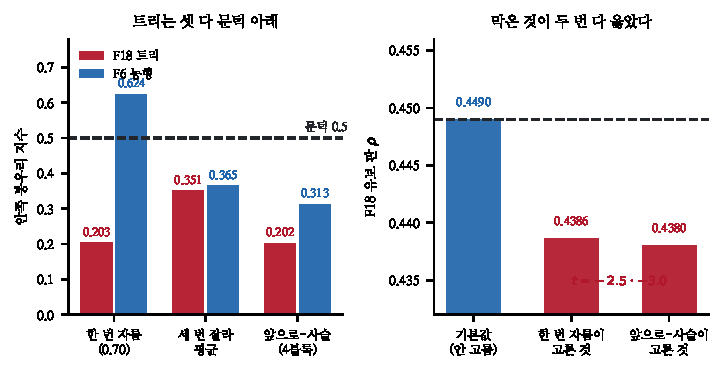
\includegraphics[width=.72\textwidth]{figs/three3.pdf}
\caption{왼쪽 --- 트리는 셋 다 문턱 아래. 오른쪽 --- 막은 것이 두 번 다
옳았다.}
\end{figure*}

\section{채점 행을 늘려도 안 된다}

\begin{table}[t]
\centering\tsize
\caption{안쪽 방식 셋.}
\begin{tabular}{lrrr}
\toprule
& 채점 행 & 트리 & 능형 \\
\midrule
한 번 자름 (0.70) & 3{,}137 & .203 & \textbf{.624} \\
세 번 잘라 평균 & --- & .351 & .365 \\
\textbf{앞으로-사슬} & \textbf{7{,}624} & .202 & \textbf{.313} \\
\bottomrule
\end{tabular}
\end{table}

\claimx{\textbf{채점 행을 2.4배로 늘렸는데 능형 봉우리가 절반으로 준다}
(.624 $\to$ .313). 잡음이 문제였다면 반대로 가야 한다.}{\textbf{노트 192의
마지막 읽기가 반증됐다} --- ``안쪽 점수가 시끄러운 것이 편향의 절반''이라고
적었는데, 시끄러움을 줄여도 안 낫는다.}

\claimx{\textbf{셋이 같은 이유로 막힌다.} 학습 크기가 다르면 최적이 진짜로
다르고, 크기를 섞는 방식은 서로 다른 봉우리를 겹쳐 평지로 만든다.}{앞으로-사슬
블록 셋의 학습행이 2,553 · 5,085 · 7,648 이다 --- \textbf{섞이는 크기 차가
세 배}다. 평균(노트 192)도 비율 0.55$\sim$0.85 로 1.7배를 섞었다.}

\section{용량은 맞췄는데 깊이가 틀렸다}

\begin{table}[t]
\centering\tsize
\caption{트리가 고른 것.}
\begin{tabular}{lrrrr}
\toprule
& 깊이 & 반복 & 학습률 & 용량 \\
\midrule
기본값 & \textbf{4} & 220 & .06 & \textbf{13.2} \\
한 번 자름 & 6 & 120 & .03 & 3.6 \\
\textbf{앞으로-사슬} & \textbf{3} & 400 & .03 & \textbf{12.0} \\
\bottomrule
\end{tabular}
\end{table}

\claimx{\textbf{사슬은 용량을 거의 맞춘다}(12.0 대 13.2). 노트 192에서 한 번
자름이 3.6 이었으니 크게 나아졌다 --- 큰 블록(7,648행)이 들어와서다.}{\textbf{그런데도
유보에서 $-$0.0110 진다}($t{=}-3.01$). 깊이를 3 으로 골랐고(기본값 4)
\textbf{그 하나가 용량을 맞춘 이득을 다 먹는다.}}

\claimx{\textbf{능형은 방식에 강건하다} --- 세 방식 전부 $\alpha{=}100$ 을
고르고 유보 $+$0.3818 로 같다.}{선형은 손잡이가 하나이고 그 하나가 학습
크기에 완만하게 반응한다. \textbf{트리는 셋이 서로 맞물려 있어 크기가
바뀌면 다른 조합으로 옮겨 간다.}}

\section{문턱이 세 번 검증됐다}

\begin{table}[t]
\centering\tsize
\caption{봉우리 지수가 막았고, 유보를 열어 보니.}
\begin{tabular}{lrrl}
\toprule
& 봉우리 & 유보 차 & \\
\midrule
한 번 자름 & .203 & $-$.0104 & 막음 · 옳음 \\
세 번 평균 & .351 & --- & 막음 \\
앞으로-사슬 & .202 & $-$.0110 & 막음 · 옳음 \\
\midrule
능형(참고) & .624 & $+$.0109 & 통과 · 옳음 \\
\bottomrule
\end{tabular}
\end{table}

\claimx{\textbf{노트 190에서 네 점 사이에 그은 문턱이 독립으로 세 번
검증됐다.} 세 방식을 다 막았고, 유보를 열어 보니 두 번 다 지는 선택이었다.
통과시킨 능형은 이기는 선택이었다.}{\textbf{규약이 값을 하는 것이 이
흐름에서 두 번째다} --- 노트 187의 ``안 움직이면 안 닿은 것''이 두 사이클
연속으로 아티팩트를 잡았고(노트 189 · 190), 봉우리 지수가 세 방식을
막았다.}

\claimx{\textbf{튜닝 갈래를 닫는다.} 능형 셋은 조정해서 $+$0.011$\sim$0.013
을 얻었고 챔피언은 이 자료로 조정할 수 없다 --- 세 방식이 다 실패했고 실패의
원인이 같다.}{판은 $+$0.4490 그대로다. \textbf{노트 189$\sim$193 다섯
사이클에서 판이 안 올랐다} --- 오른 것은 도전자 셋이고 챔피언은 안
움직였다.}

\begin{table}[t]
\centering\tsize
\caption{남은 것.}
\begin{tabular}{ll}
\toprule
\textbf{크기 고정} & 블록마다 학습행을 같게 자르면 \\
깊이 & 용량과 따로 다뤄야 하나 \\
\textbf{다음 갈래} & 튜닝 말고 --- 자료로 돌아갈 것 \\
\bottomrule
\end{tabular}
\end{table}

첫 줄이 이 갈래에서 마지막으로 남은 것이다. 크기 혼합이 원인이라면
\emph{크기를 고정}하면 된다 --- 블록마다 앞에서부터 다 쓰는 대신 \emph{창을
밀며} 늘 같은 행 수로 적합하는 것이다. 그러면 봉우리가 설 수 있다. 다만
그때 학습행은 제일 작은 블록에 맞춰야 하므로 2,553 행이 되고, 전체 학습
10,292 행과 네 배 차이라 \textbf{노트 192가 잰 용량 편향이 더 커진다.}
\textbf{어느 쪽으로도 빠져나갈 곳이 없어 보이고, 그래서 다음 사이클은
튜닝이 아니라 자료로 돌아간다.}

\end{document}
